%!TEX program = xelatex
%\documentclass[UTF8]{ctexart}

\documentclass[UTF8]{beamer}
\usepackage{ulem}
\usepackage{graphicx}
\usepackage{fontspec} 
\usepackage{xeCJK} 
\usepackage{bm, amsmath}
\usepackage{mathrsfs} %支持花体字母
\usetheme{Warsaw}
\title[ACM Class Compiler2016]{The Compiler Of Language MFChen}
\author{Bai YiWei}
\date{May 10, 2016}
\newtheorem{obs}{Observation}
\setcounter{obs}{1}
\AtBeginSubsection[]
{
	\begin{frame}<beamer>{Outline}
		\tableofcontents[currentsection,currentsubsection]
	\end{frame}
}

\begin{document}

\begin{frame}
\titlepage
\end{frame}

\begin{frame}{词法分析和语法分析}
	\begin{itemize}
	\item 使用Antlr4来完成词法分析和语法分析
	\item 处理运算符优先级方法如下(\sout{未充分利用Antlr4特性})
	\end{itemize}
	\begin{figure}[!htb]
	\centering
	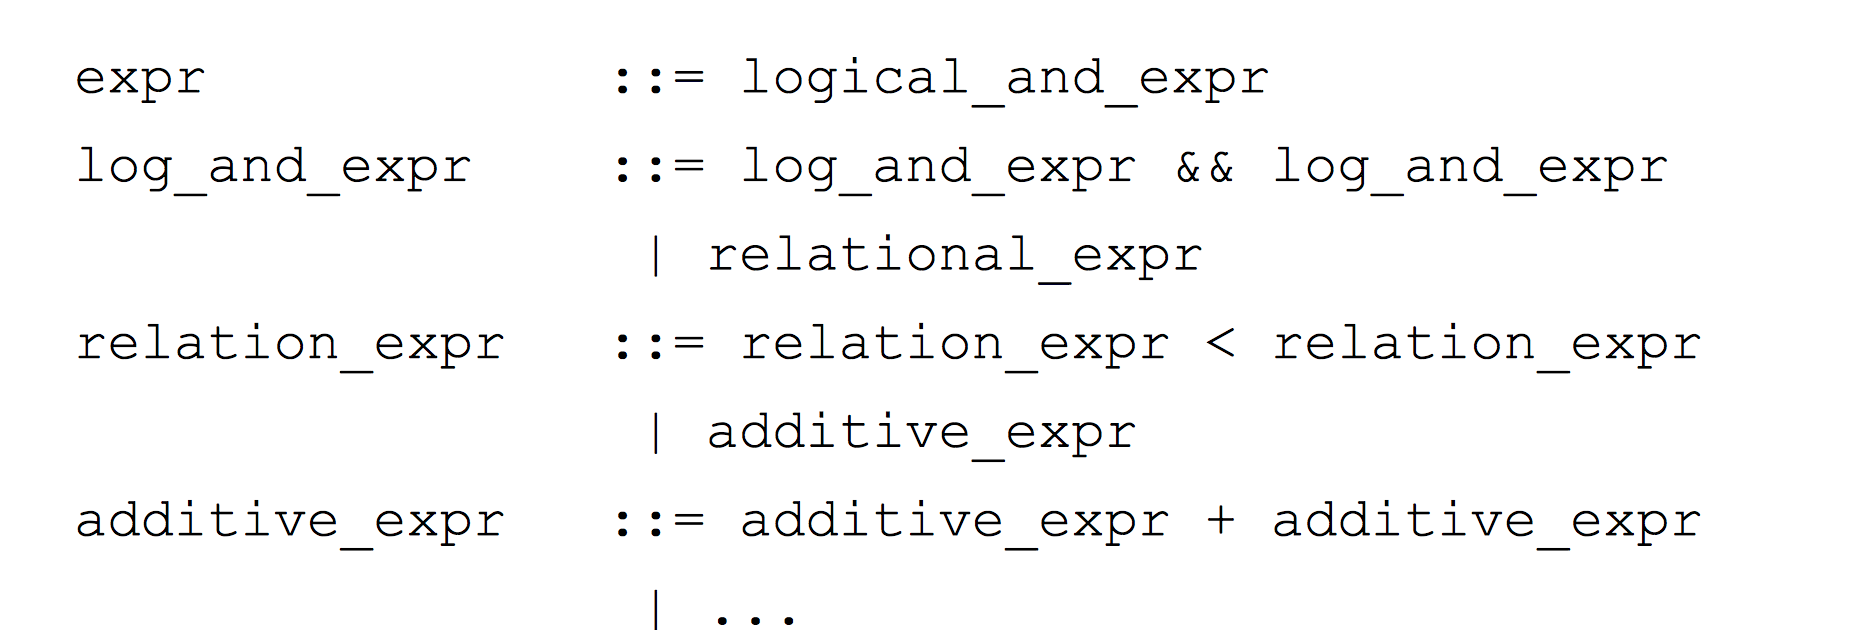
\includegraphics[width=0.6\textwidth]{1.png}
	%\caption{标题}
	\end{figure}
\end{frame}

\begin{frame}{符号表}
	\begin{itemize}
	\item 基本思路是虎书的符号表(双链表实现)
	\item 对于每一个Symbol,需要存$pair<scope, Property>$
	\end{itemize}
\end{frame}

\begin{frame}{\sout{AST}CST}
	\begin{itemize}
	\item Antlr4的Visitor下,CST跟AST没有本质差别
	\item 非常遗憾没能借助AST练习下设计模式的一些东西T-T
	\end{itemize}
\end{frame}

\begin{frame}{语义分析}
	扫微小的三遍
	\begin{itemize}
	\item 处理出所有可能的Type(用户定义的Class)
	\item 处理出函数的性质和Class性质
	\item 检查程序语义
	\end{itemize}
\end{frame}

\begin{frame}{中间表示}
	\begin{itemize}
	\item 采用Eac ILOC规范的三地址码
	\item 既然有了无限寄存器,那么要load store指令有和用?
	\item 魔改了一下,对虚拟寄存器进行了分类 $\quad \Rightarrow \quad$ 大锅
	\end{itemize}
\end{frame}

\begin{frame}{代码生成}
	\begin{itemize}
	\item 先写一个Memory to Memory内存模型的程序,简单、易查错
	\item 程序架构完全靠自己思考,后期转换困难
	\end{itemize}
\end{frame}

\begin{frame}{内建函数实现}
	\begin{itemize}
	\item 全部自己手写MIPS实现,采用内联方式
	\item 感受到了汇编语言不一样的思维
	\end{itemize}
\end{frame}

\begin{frame}{\sout{Cache}}
	\begin{itemize}
	\item 为什么不能拿寄存器当缓存来实现一下Cache呢?
	\item 先对每个基本块按照使用频率分配寄存器,当不够的时候踢掉前面那个使用频率最低的
	\end{itemize}
\end{frame}

\begin{frame}{魔改的代价}
	\begin{itemize}
	\item 调不对T-T
	\end{itemize}
\end{frame}

\begin{frame}{Memory To Memory 相关优化}
	\begin{itemize}
	\item 利用寄存器多的用不了,优化MIPS伪指令 e.g $li$
	\item 分析每一个基本快的无用load、store进行删除
	\end{itemize}
\end{frame}

\begin{frame}{PrettyPrint}
	\begin{itemize}
	\item 在CST上走一遍即可实现,利用scope处理缩进问题
	\end{itemize}
\end{frame}

\begin{frame}{丑陋的代码}
	\begin{figure}[htpb]
	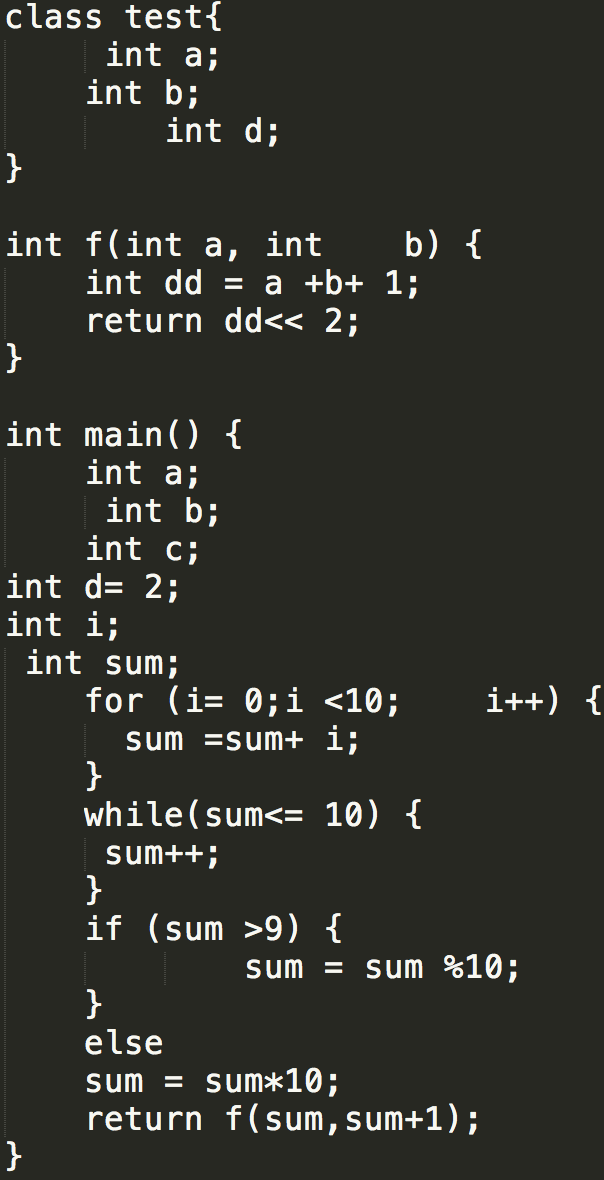
\includegraphics[width=0.4\textwidth]{2.png}
	%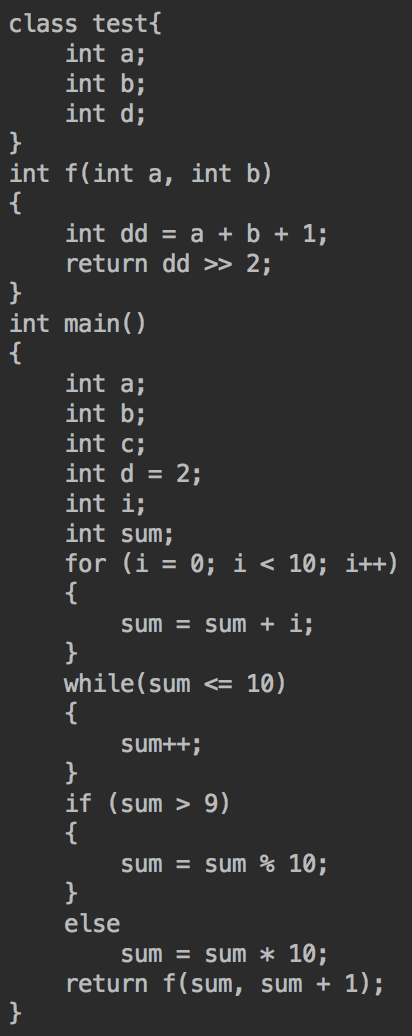
\includegraphics[width=0.4\textwidth]{3.png}
	%\caption{标题}
	\end{figure}
\end{frame}

\begin{frame}{PrettyPrint后的代码}
	\begin{figure}[htpb]
	%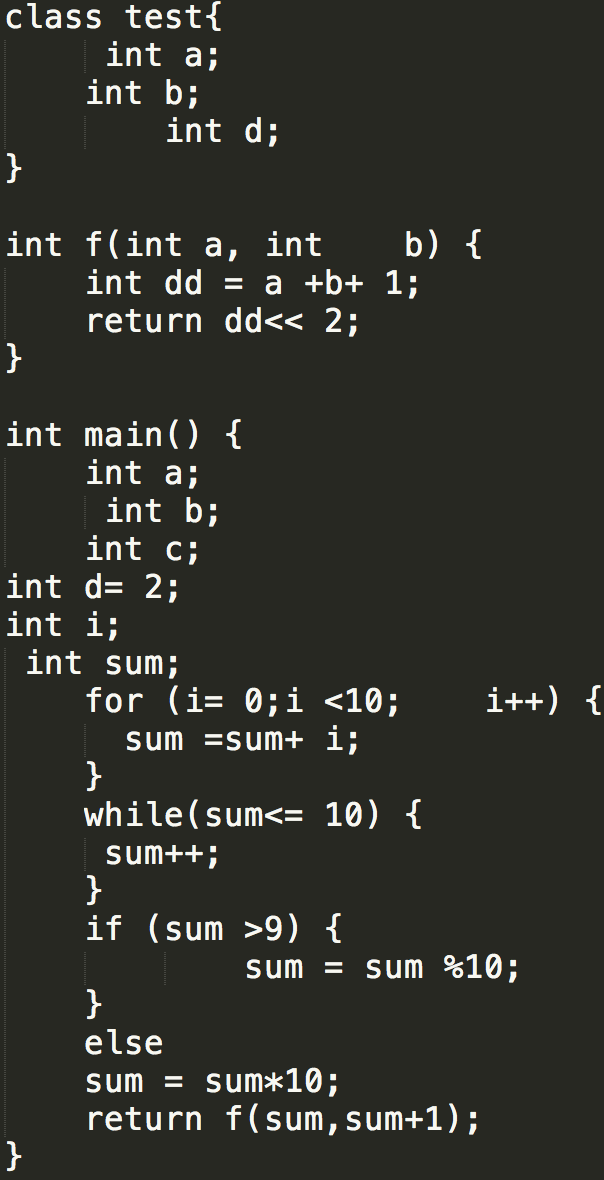
\includegraphics[width=0.5\textwidth]{2.png}
	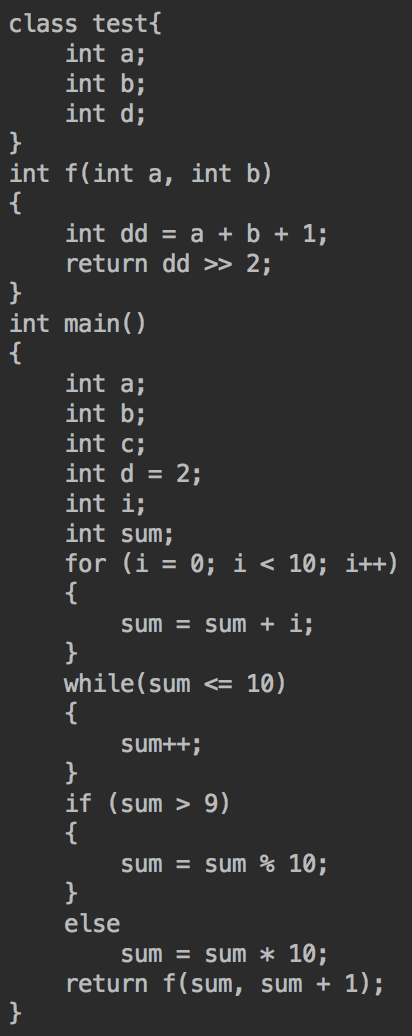
\includegraphics[width=0.3\textwidth]{3.png}
	%\caption{标题}
	\end{figure}
\end{frame}

\begin{frame}{感想}

\end{frame}

\begin{frame}
	\begin{itemize}
	\item 感谢马老师的课程
	\item 感谢助教们的努力工作和对我们的帮助
	\end{itemize}
\end{frame}